%!TEX root = ./EpsilonBook.tex

\chapter{The Epsilon Object Language (EOL)}
\label{sec:Design.EOL}

The primary aim of EOL is to provide a reusable set of common model management facilities, atop which task-specific languages can be implemented. However, EOL can also be used as a general-purpose standalone model management language for automating tasks that do not fall into the patterns targeted by task-specific languages. This section presents the syntax and semantics of the language using a combination of abstract syntax diagrams, concrete syntax examples and informal discussion.

\section{Module Organization}
\label{sec:Design.EOL.Syntax}
\label{sec:Design.EOL.ModuleStucture}

In this section the syntax of EOL is presented in a top-down manner. As displayed in Figure \ref{fig:EOL.Module}, EOL programs are organized in \emph{modules}. Each module defines a \emph{body} and a number of \emph{operations}. The body is a block of statements that are evaluated when the module is executed\footnote{Although the EOL parser permits loose statements (e.g. not contained in operations) between/after operations, these are ignored at runtime.}. Each operation defines the kind of objects on which it is applicable (\emph{context}), a \emph{name}, a set of \emph{parameters} and optionally a \emph{return type}. Modules can also import other modules using \emph{import} statements and access their operations, as shown in Listing~\ref{lst:ExampleImports}.

\begin{sidewaysfigure}
  \centering
  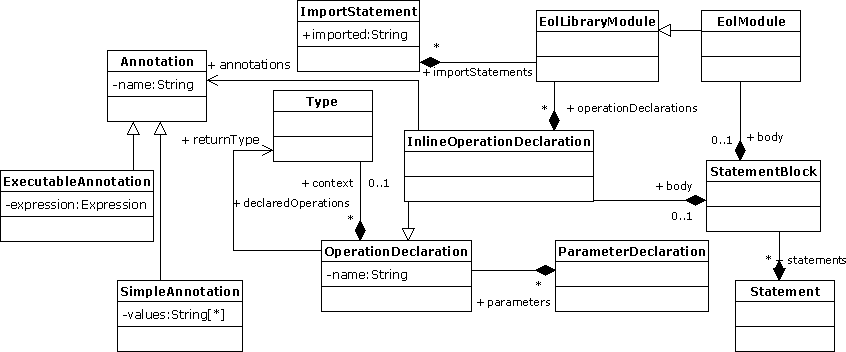
\includegraphics[width=\textwidth,height=\textheight,keepaspectratio]{images/EOLModule.png}
  \caption{EOL Module Structure}
  \label{fig:EOL.Module}
\end{sidewaysfigure}

\begin{lstlisting}[float, caption={Example of two related EOL modules}, label=lst:ExampleImports, language=EOL]
// file imported.eol
operation hello() {
  'Hello world!'.println();
}

// file importer.eol
// We can use relative/absolute paths or platform:/ URIs
import "imported.eol";

hello(); // main body

// ... more operations could be placed here ...
\end{lstlisting}

\section{User-Defined Operations}
\label{sec:Design.EOL.Operations}

In typical object oriented languages such as Java and C++, operations are defined inside classes and can be invoked on instances of those classes. EOL on the other hand is not object-oriented in the sense that it does not define classes itself, but nevertheless needs to manage objects of types defined externally to it (e.g. in metamodels). By defining the context-type of an operation explicitly, the operation can be called on instances of the type as if it was natively defined by the type. Alternatively, context-less operations could be defined; however the adopted technique significantly improves readability of the concrete syntax.

For example, consider the code excerpts displayed in Listings \ref{lst:OperationsContext} and \ref{lst:OperationsNoContext}. In Listing \ref{lst:OperationsContext}, the operations \emph{add1} and \emph{add2} are defined in the context of the built-in \emph{Integer} type, which is specified before their names. Therefore, they can be invoked in line 1 using the \emph{1.add1().add2()} expression: the context (the integer \emph{1}) will be assigned to the special variable \emph{self}. On the other hand, in Listing \ref{lst:OperationsNoContext} where no context is defined, they have to be invoked in a nested manner which follows an in-to-out direction instead of the left to right direction used by the former excerpt. As complex model queries often involve invoking multiple properties and operations, this technique is particularly beneficial to the overall readability of the code.

\begin{lstlisting}[float=tbp, caption={Context-defining EOL operations}, label=lst:OperationsContext, language=EOL]
1.add1().add2().println();

operation Integer add1() : Integer {
	return self + 1;
}

operation Integer add2() : Integer {
	return self + 2;
}
\end{lstlisting}

\begin{lstlisting}[float=tbp, caption={Context-less EOL operations}, label=lst:OperationsNoContext, language=EOL]
add2(add1(1)).println();

operation add1(base : Integer) : Integer {
	return base + 1;
}

operation add2(base : Integer) : Integer {
	return base + 2;
}
\end{lstlisting}

EOL supports polymorphic operations using a runtime dispatch mechanism. Multiple operations with the same name and parameters can be defined, each defining a distinct context type. For example, in Listing \ref{lst:Polymorphism}, the statement in line 1 invokes the test operation defined in line 4, while the statement in line 2 invokes the test operation defined in line 8.

\begin{lstlisting}[float=tbp, caption=Demonstration of polymorphism in EOL, label=lst:Polymorphism, numbers=left, language=EOL]
"1".test();
1.test();

operation String test() {
	(self + " is a string").println();
}

operation Integer test() {
	(self + "is an integer").println();
}

\end{lstlisting}

\subsection{Annotations}
\label{sec:Design.EOL.Annotations}
EOL supports two types of annotations: simple and executable. A simple annotation specifies a name and a set of String values while an executable annotation specifies a name and an expression. The concrete syntaxes of simple and executable annotations are displayed in Listings \ref{lst:SimpleAnnotations} and \ref{lst:ExecutableAnnotations} respectively. Several examples for simple annotations are shown in Listing~\ref{lst:SimpleAnnotationsExamples}. Examples for executable annotations will be given in the following sections.

\begin{lstlisting}[float=tbp, caption=Concrete syntax of simple annotations, label=lst:SimpleAnnotations, language=EOL, escapechar=!]
!\textbf{@}!name value(,value)*
\end{lstlisting}

\begin{lstlisting}[float=tbp, caption=Concrete syntax of executable annotations, label=lst:ExecutableAnnotations, language=EOL, escapechar=!]
!\textbf{\$}!name expression
\end{lstlisting}

\begin{lstlisting}[float=tbp, caption=Examples of simple annotations, label=lst:SimpleAnnotationsExamples, language=EOL, escapechar=!]
!\textbf{@}!colors red
!\textbf{@}!colors red, blue
!\textbf{@}!colors red, blue, green
\end{lstlisting}

In stand-alone EOL, annotations are supported only in the context of operations, however as discussed in the sequel, task-specific languages also make use of annotations in their constructs, each with task-specific semantics. EOL operations support three particular annotations: the \emph{pre} and \emph{post} executable annotations for specifying pre and post-conditions, and the \emph{cached} simple annotation, which are discussed below.

\subsection{Pre/post conditions in user-defined operations}
\label{sec:prep-cond-user}

A number of \emph{pre} and \emph{post} executable annotations can be attached to EOL operations to specify the pre- and post-conditions of the operation. When an operation is invoked, before its body is evaluated, the expressions of the \emph{pre} annotations are evaluated. If all of them return \emph{true}, the body of the operation is processed, otherwise, an error is raised. Similarly, once the body of the operation has been executed, the expressions of the \emph{post} annotations of the operation are executed to ensure that the operation has had the desired effects. \emph{Pre} and \emph{post} annotations can access all the variables in the parent scope, as well as the parameters of the operation and the object on which the operation is invoked (through the \emph{self} variable). Moreover, in \emph{post} annotations, the returned value of the operation is accessible through the built-in \emph{\_result} variable. An example of using pre and post conditions in EOL appears in Listing \ref{lst:PrePostConditionsExample}.

\begin{lstlisting}[float=tbp, caption=Example of pre- and post-conditions in an EOL operation, label=lst:PrePostConditionsExample, language=EOL]
1.add(2); /*@\label{line:ConditionsOK}@*/
1.add(-1); /*@\label{line:PreConditionFails}@*/

$pre i > 0 /*@\label{line:PreCondition}@*/
$post _result > self /*@\label{line:PostCondition}@*/
operation Integer add(i : Integer) : Integer {
	return self + i;
}
\end{lstlisting}

In line \ref{line:PreCondition} the \emph{add} operation defines a pre-condition stating that the parameter \emph{i} must be a positive number. In line \ref{line:PostCondition}, the operation defines that result of the operation (\emph{\_result}) must be greater than the number on which it was invoked (\emph{self}). Thus, when executed in the context of the statement in line \ref{line:ConditionsOK} the operation succeeds, while when executed in the context of the statement in line \ref{line:PreConditionFails}, the pre-condition is not satisfied and an error is raised. 

\subsection{Operation Result Caching}
\label{sec:EolCaching}

EOL supports caching the results of parameter-less operations using the \emph{@cached} simple annotation. In the following example, the Fibonacci number of a given Integer is calculated using the \emph{fibonacci} recursive operation displayed in Listing \ref{lst:Fibonacci}. Since the \emph{fibonacci} operation is declared as \emph{cached}, it is only executed once for each distinct Integer and subsequent calls on the same target return the cached result. Therefore, when invoked in line \ref{line:FibonnaciCall}, the body of the operation is called 16 times. By contrast, if no \emph{@cached} annotation was specified, the body of the operation would be called recursively 1973 times. This feature is particularly useful for performing queries on large models and caching their results without needing to introduce explicit variables that store the cached results.

Note that the cached result is not copied before it is returned, this has some implecations for returned lists of objects. For example, if a returned Set is modified, next time this modfied Set is returned instead of the original Set. If the Set needs to be modfied, first copy its contents into a new local Set.

\begin{lstlisting}[float=tbp, caption=Calculating the Fibonacci number using a cached operation, label=lst:Fibonacci, language=EOL]
15.fibonacci().println(); /*@\label{line:FibonnaciCall}@*/

@cached
operation Integer fibonacci() : Integer {
	if (self = 1 or self = 0) {
		return 1;
	}
	else {
		return (self-1).fibonacci() + (self-2).fibonacci();
	}
}
\end{lstlisting}

\section{Types}
\label{sec:eol_types}

As is the case for most programming languages, EOL defines a built-in system of types, illustrated in Figure \ref{fig:EOLTypes}. The \emph{Any} type, inspired by the \emph{OclAny} type of OCL, is the basis of all types in EOL including Collection types. The operations supported by instances of the Any type are outlined in Table \ref{tab:AnyOperations}\footnote{Parameters within square braces [ ] are optional}.

\begin{figure}[t]
  \centering
  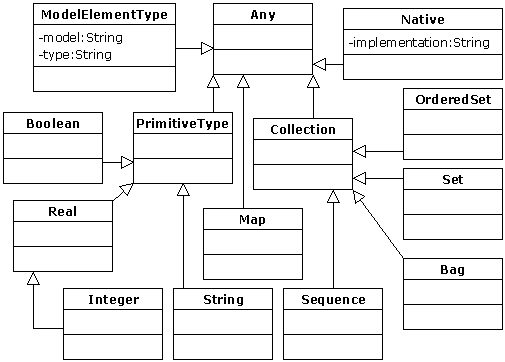
\includegraphics{images/EOLTypes.png}
  \caption{Overview of the type system of EOL}
  \label{fig:EOLTypes}
\end{figure}

\clearpage

\begin{longtabu} {|p{6.5cm}|X|}
			
			\caption{Operations of type Any}
			\label{tab:AnyOperations}\\
			
			\hline
							
			\textbf{Signature} & \textbf{Description} \\\hline

			isDefined() : Boolean & Returns true if the object is defined and false otherwise \\\hline
			
			isUndefined() : Boolean & Returns true if the object is undefined and false otherwise \\\hline
			
			ifUndefined(alt : Any) : Any & If the object is undefined, it returns alt else it returns the object \\\hline
			
			isTypeOf(type : Type) : Boolean & Returns true if the object is of the given type and false otherwise \\\hline
			
			isKindOf(type : Type) : Boolean & Returns true if the object is of the given type or one of its subtypes and false otherwise \\\hline
			
			type() : Type & Returns the type of the object. The EOL type system is illustrated in Figure \ref{fig:EOLTypes} \\\hline

                        owningModel() : Model & Returns the model that contains this object or an undefined value otherwise \\\hline

                        hasProperty(name : String) : Boolean & Returns true if the object has a property with the specified name or false otherwise \\\hline
                        
			asString() : String & Returns a string representation of the object \\\hline
			
			asInteger() : Integer & Returns an Integer based on the string representation of the object. If the string representation is not of an acceptable format, an error is raised \\\hline
			
			asReal() : Real & Returns a Real based on the string representation of the object. If the string representation is not of an acceptable format, an error is raised \\\hline
			
			asBoolean() : Boolean & Returns a Boolean based on the string representation of the object. If the string representation is not of an acceptable format, an error is raised \\\hline
			
			asBag() : Bag & Returns a new Bag containing the object \\\hline
			
			asSequence() : Sequence & Returns a new Sequence containing the object \\\hline
			
			asSet() : Set & Returns a new Set containing the object \\\hline
			
			asOrderedSet() : OrderedSet & Returns a new OrderedSet containing the object \\\hline
			
			print([prefix : String]) : Any & Prints a string representation of the object on which it is invoked to the regular output stream, prefixed with the optional \emph{prefix} string and returns the object on which it was invoked. In this way, the \emph{print} operation can be used for debugging purposes in a non-invasive manner\\\hline
			
			println([prefix : String]) : Any & Has the same effects as the \emph{print} operation but also produces a new line in the output stream. \\\hline

			err([prefix : String]) : Any & Prints a string representation of the object on which it is invoked to the error stream prefixed with the optional \emph{prefix} string and returns the object on which it was invoked. In this way, the \emph{print} operation can be used for debugging purposes in a non-invasive manner\\\hline
			
			errln([prefix : String]) : Any & Has the same effects as the \emph{err} operation but also produces a new line in the output stream. \\\hline
			
			format([pattern : String]) : String & Uses the provided pattern to form a String representation of the object on which the method is invoked. The pattern argument must conform to the format string syntax defined by Java\footnote{\url{http://download.oracle.com/javase/6/docs/api/java/util/Formatter.html\#syntax}}. \\\hline

\end{longtabu}

\subsection{Primitive Types} 

EOL provides four primitive types: String, Integer, Real and Boolean. The String type represents finite sequences of characters and supports the following operations which can be invoked on its instances.

\begin{longtabu} {|p{6.5cm}|X|}
			
			\caption{Operations of type String}
			\label{tab:StringOperations}\\
			
			\hline 
							
			\textbf{Signature} & \textbf{Description} \\\hline
			
			charAt(index : Integer) : String & Returns the character in the specified index\\\hline
			
			concat(str : String) : String & Returns a concatenated form of the string with the \emph{str} parameter\\\hline

			length() : Integer & Returns the number of characters in the string \\\hline
						
			toLowerCase() : String & Returns a new string where all the characters have been converted to lower case\\\hline
			
			firstToLowerCase() : String & Returns a new string the first character of which has been converted to lower case \\\hline
			
			toUpperCase() : String & Returns a new string where all the characters have been converted to upper case\\\hline
			
			firstToUpperCase() : String & Returns a new string, the first character of which has been converted to upper case \\\hline
			
			isSubstringOf(str : String) : Boolean & Returns true iff the string the operation is invoked on is a substring of \emph{str} \\\hline
			
			matches(reg : String) : Boolean & Returns true if there are occurrences of the regular expression \emph{reg} in the string\\\hline
			
			replace(source : String, target : String) : String & Returns a new string in which all instances of \emph{source} have been replaced with instances of \emph{target}\\\hline 
			
			split(reg : String) : Sequence(String) & Splits the string using as a delimiter the provided regular expression, \emph{reg}, and returns a sequence containing the parts\\\hline
			
			startsWith(str : String) : Boolean & Returns true iff the string starts with \emph{str}\\\hline
			
			endsWith(str : String) : Boolean & Returns true iff the string ends with \emph{str}\\\hline

			isInteger() : Boolean & Returns true iff the string is an integer\\\hline
			
			isReal() : Boolean & Returns true iff the string is a real number\\\hline
						
			toCharSequence() : Sequence(String) & Returns a sequence containing all the characters of the string\\\hline
			
			substring(index : Integer) : String & Returns a sub-string of the string starting from the specified \emph{index} and extending to the end of the original string\\\hline
			
			substring(startIndex : Integer, endIndex : Integer) : String & Returns a sub-string of the string starting from the specified \emph{startIndex} and ending at \emph{endIndex} \\\hline
			
			pad(length : Integer, padding : String, right : Boolean) : String & Pads the string up to the specified length with specified padding (e.g. "foo".pad(5, "*", true) returns "foo**") \\\hline
			
			trim() : String & Returns a trimmed copy of the string \\\hline			
			
\end{longtabu}

The Real type represents real numbers and provides the following operations.

\begin{longtabu} {|p{6.5cm}|X|}
			
			\caption{Operations of type Real}
			\label{tab:RealOperations}\\
			
			\hline
			
			\textbf{Signature} & \textbf{Description} \\\hline

			ceiling() : Integer & Returns the nearest Integer that is larger than the real\\\hline
			
			floor() : Integer & Returns the nearest Integer that is greater than the real\\\hline
			
			round() : Integer & Rounds the real to the nearest Integer\\\hline
			
			pow(exponent : Real) : Real & Returns the real to the power of exponent \\\hline
			
			log() : Real & Returns the natural logarithm of the real \\\hline
			
			log10() : Real & Returns the 10-based logarithm of the real \\\hline 
			
			abs() : Real & Returns the absolute value of the real \\\hline
			
			max(other : Real) : Real & Returns the maximum of the two reals \\\hline
			
			min(other : Real) : Real & Returns the minimum of the two reals \\\hline
			
\end{longtabu}

The Integer type represents natural numbers and negatives and extends the Real primitive type. It also defines the following operations:

\begin{longtabu} {|p{6.5cm}|X|}
			
			\caption{Operations of type Integer}
			\label{tab:IntegerOperations}\\
			
			\hline
							
			\textbf{Signature} & \textbf{Description} \\\hline

			to(other : Integer) : Sequence(Integer) & Returns a sequence of integers (e.g. 1.to(5) returns Sequence\{1,2,3,4,5\})\\\hline
			
			iota(end : Integer, step : Integer) : Sequence(Integer) & Returns a sequence of integers up to \emph{end} using the specified step (e.g. 1.iota(10,2) returns Sequence\{1,3,5,7,9\})\\\hline
			
\end{longtabu}

Finally, the Boolean type represents true/false states and provides no additional operations to those provided by the base Any type.

\subsection{Collections and Maps} 
\label{sec:Design.EOL.Collections}

EOL provides four types of collections and a Map type. The Bag type represents non-unique, unordered collections, the Sequence type represents non-unique, ordered collections, the Set type represents unique and unordered collections and the OrderedSet represents unique and ordered collections.

All collection types inherit from the abstract Collection type. Apart from simple operations, EOL also supports first-order logic operations on collections. The following operations apply to all types of collections:

\begin{longtabu} {|p{6.5cm}|X|}
			
			\caption{Operations of type Collection}
			\label{tab:Collection Operations}\\
			
			\hline
							
			\textbf{Signature} & \textbf{Description} \\\hline

			add(item : Any) & Adds an item to the collection. If the collection is a set, addition of duplicate items has no effect \\\hline
			
			addAll(col : Collection) & Adds all the items of the \emph{col} argument to the collection. If the collection is a set, it only adds items that do not already exist in the collection\\\hline
		
			remove(item : Any) & Removes an \emph{item} from the collection \\\hline
			
			removeAll(col : Collection) & Removes all the items of \emph{col} from the collection \\\hline
			
			clear() & Empties the collection \\\hline
			
			includes(item : Any) : Boolean & Returns true if the collection includes the \emph{item} \\\hline
			
			excludes(item : Any) : Boolean & Returns true if the collection excludes the \emph{item} \\\hline
			
			includesAll(col : Collection) : Boolean & Returns true if the collection includes all the items of collection \emph{col} \\\hline
			
			excludesAll(col : Collection) : Boolean & Returns true if the collection excludes all the items of collection col \\\hline
			
			including(item : Any) : Collection & Returns a new collection that also contains the \emph{item} -- unlike the add() operation that adds the \emph{item} to the collection itself  \\\hline
			
			excluding(item : Any) : Collection & Returns a new collection that excludes the item -- unlike the remove() operation that removes the \emph{item} from the collection itself\\\hline
			
			includingAll(col : Collection) : Collection & Returns a new collection that is a union of the two collections. The type of the returned collection (i.e. Bag, Sequence, Set, OrderedSet) is same as the type of the collection on which the operation is invoked \\\hline
			
			excludingAll(col : Collection) : Collection & Returns a new collection that excludes all the elements of the col collection \\\hline
			
			flatten() : Collection & Recursively flattens all items that are of collection type and returns a new collection where no item is a collection itself \\\hline
			
			count(item : Any) : Integer & Returns the number of times the item exists in the collection \\\hline
			
			size() : Integer & Returns the number of items the collection contains \\\hline

			sum() : Real & Returns the sum of all reals/integers in the collection\\\hline

			product() : Real & Returns the product of all reals/integers in the collection\\\hline
			
			isEmpty() : Boolean & Returns true if the collection does not contain any elements and false otherwise \\\hline
	
			random() : Any & Returns a random item from the collection \\\hline
			
			clone() : Collection & Returns a new collection of the same type containing the same items with the original collection \\\hline
			
			concat() : String & Returns the string created by converting each element of the collection to a string \\\hline
			
			concat(separator : String) : String & Returns the string created by converting each element of the collection to a string, using the given argument as a separator \\\hline
\end{longtabu}

The following operations apply to ordered collection types (i.e. Sequence and OrderedSet):

\begin{longtabu} {|p{6.5cm}|X|}
			
			\caption{Operations of types Sequence and OrderedSet}
			\label{tab:SortedOperations}\\
			
			\hline
							
			\textbf{Signature} & \textbf{Description} \\\hline

			first() : Any & Returns the first item of the collection  \\\hline

			second() : Any & Returns the second item of the collection  \\\hline

			third() : Any & Returns the third item of the collection  \\\hline

			fourth() : Any & Returns the fourth item of the collection  \\\hline
				
			last() : Any & Returns the last item of the collection  \\\hline
	
			at(index : Integer) : Any & Returns the item of the collection at the specified index \\\hline
			
			removeAt(index : Integer) : Any & Removes and returns the item at the specified index. \\\hline
			
			indexOf(item : Any) : Integer & Returns the index of the item in the collection or -1 if it does not exist \\\hline

			invert() : Collection & Returns an inverted copy of the collection\\\hline
						
\end{longtabu}

Also, EOL collections support the following first-order operations:

\begin{longtabu} {|p{6.5cm}|X|}
			
			\caption{First-order logic operations on Collections}
			\label{tab:FirstOrderOperations}\\
			
			\hline
							
			\textbf{Signature} & \textbf{Description} \\\hline

			select(iterator : Type $|$ condition) : Collection & Returns a sub-collection containing only items of the specified type that satisfy the condition \\\hline 

			selectOne(iterator : Type $|$ condition) : Any & Returns the first element that satisfies the condition \\\hline
			
			reject(iterator : Type $|$ condition) : Collection & Returns a sub-collection containing only items of the specified type that do not satisfy the condition \\\hline
			
			collect(iterator : Type $|$ expression) : Collection &  Returns a collection containing the results of evaluating the expression on each item of the collection that is of the specified type \\\hline

                        closure(iterator : Type $|$ expression) : Collection & Returns a collection containing the results of evaluating the transitive closure of the results produced by the expression on each item of the collection that is of the specified type \\\hline

                        aggregate(iterator : Type $|$ keyExpression, valueExpression) : Map & Returns a map containing key-value pairs produced by evaluating the key and value expressions on each item of the collection that is of the specified type \\\hline

			one(iterator : Type $|$ condition) : Boolean & Returns true if there exists exactly one item in the collection that satisfies the condition \\\hline

			exists(iterator : Type $|$ condition) : Boolean & Returns true if there exists at least one item in the collection that satisfies the condition \\\hline
			
			forAll(iterator : Type $|$ condition) : Boolean & Returns true if all items in the collection satisfy the condition \\\hline
			
			%iterate(iterator : IteratorType ; result : ResultType = initialValue $|$ expression) : ResultType & Iterates all the items of the collection that conform to the IteratorType and incrementally calculates the value of the result variable which it finally returns \\\hline
			
			sortBy(iterator: Type $|$ expression) : Collection & Returns a copy of the collection sorted by the results of evaluating the expression on each item of the collection that conforms to the iterator type \\\hline

\end{longtabu}

The Map type represents an array of key-value pairs in which the keys are unique. The type provides the following operations.

\begin{longtabu} {|p{6.5cm}|X|}
			
			\caption{Operations of type Map}
			\label{tab:MapOperations}\\
			
			\hline
			
			\textbf{Signature} & \textbf{Description} \\\hline

			put(key : Any, value : Any) & Adds the key-value pair to the map. If the map already contains the same key, the value is overwritten\\\hline
				
			get(key : Any) : Any & Returns the value for the specified keys\\\hline
	
			containsKey(key : Any) : Boolean & Returns true if the map contains the specified key\\\hline
	
			keySet() : Set & Returns the keys of the map\\\hline
			
			values() : Bag & Returns the values of the map\\\hline
			
			clear() & Clears the map\\\hline
			
\end{longtabu}

\subsection{Native Types}

As discussed earlier, while the purpose of EOL is to provide significant expressive power to enable users to manage models at a high level of abstraction, it is not intended to be a general-purpose programming language. Therefore, there may be cases where users need to implement some functionality that is either not efficiently supported by the EOL runtime (e.g. complex mathematical computations) or that EOL does not support at all (e.g. developing user interfaces, accessing databases). To overcome this problem, EOL enables users to create objects of the underlying programming environment by using \emph{native} types. A native type specifies an $implementation$ property that indicates the unique identifier for an underlying platform type. For instance, in a Java implementation of EOL the user can instantiate and use a Java class via its class identifier. Thus, in Listing \ref{lst:Native} the EOL excerpt creates a Java window (Swing JFrame) and uses its methods to change its title and dimensions and make it visible.

\begin{lstlisting}[float=tbp, caption=Demonstration of NativeType in EOL, label=lst:Native, language=EOL]
var frame = new Native("javax.swing.JFrame");
frame.title = "Opened with EOL";
frame.setBounds(100,100,300,200);
frame.visible = true;
\end{lstlisting}

To pass arguments to the constructor of a native type, a parameter list must be added, such as that in Listing~\ref{lst:Native-params}.

\begin{lstlisting}[float=tbp, caption=Demonstration of NativeType in EOL, label=lst:Native-params, numbers=left, language=EOL]
var file = new Native("java.io.File")("myfile.txt");
file.absolutePath.println();
\end{lstlisting}

\subsection{Model Element Types}

A model element type represents a meta-level classifier. As discussed in Section \ref{sec:Design.EMC}, Epsilon intentionally refrains from defining more details about the meaning of a model element type to be able to support diverse modelling technologies where a type has different semantics. For instance a MOF class, an XSD complex type and a Java class can all be regarded as model element types according to the implementation of the underlying modelling framework.

In case of multiple models, as well as the name of the type, the name of the model is also required to resolve a particular type since different models may contain elements of homonymous but different model element types. In case a model defines more than one type with the same name (e.g. in different packages), a fully qualified type name must be provided.

In terms of concrete syntax, inspired by ATL, the ! character is used to separate the name of the type from the name of the model it is defined in. For instance $Ma!A$ represents the type $A$ of model $Ma$. Also, to support modelling technologies that provide hierarchical grouping of types (e.g. using packages) the :: notation is used to separate between packages and classes.  A model element type supports the following operations:

\begin{longtabu} {|p{6.5cm}|X|}
			
			\caption{Operations of Model Element Types}
			\label{tab:ModelElementTypesOperations}\\
			
			\hline
			
			\textbf{Signature} & \textbf{Description} \\\hline
			
			allOfType() : Set & Returns all the elements in the model that are instances of the type \\\hline
			
			allOfKind() : Set & Returns all the elements in the model that are instances either of the type itself or of one of its subtypes  \\\hline

			allInstances() : Set & Alias for allOfKind() (for compatibility with OCL) \\\hline
						
			all() : Set & Alias for allOfKind() (for syntax-compactness purposes) \\\hline
			
			isInstantiable() : Boolean & Returns true if the type is instantiable (i.e. non-abstract)  \\\hline
			
			createInstance() : Any & Creates an instance of the type in the model \\\hline
			
\end{longtabu}

As an example of the concrete syntax, Listing \ref{lst:ModelElementTypes} retrieves all the instances of the Class type (including instances of its subtypes) defined in the Core package of the UML 1.4 metamodel that are contained in the model named UML14.

\begin{lstlisting}[float=tbp, caption=Demonstration of the concrete syntax for accessing model element types, label=lst:ModelElementTypes, language=EOL]
UML14!Core::Foundation::Class.allInstances();
\end{lstlisting}

\section{Expressions}

\subsection{Literal Values}

EOL provides special syntax constructs to create instances of each of the built-in types:

\begin{description}
\item[Integer] literals are defined by using one or more decimal
  digits (such as \emph{42} or \emph{999}). Optionally, long integers
  (with the same precision as a Java \emph{Long}) can be produced by
  adding a ``l'' suffix, such as \emph{42l}.

\item[Real] literals are defined by:
  \begin{itemize}
  \item Adding a decimal separator and non-empty fractional part to
    the integer part, such as \emph{42.0} or \emph{3.14}. Please note
    that \emph{.2} and \emph{2.} are \emph{not} valid literals.
  \item Adding a floating point suffix: ``f'' and ``F'' denote single
    precision, and ``d'' and ``D'' denote double precision. For
    example, \emph{2f} or \emph{3D}.
  \item Adding an exponent, such as \emph{2e+1} (equal to \emph{2e1})
    or \emph{2e-1}.
  \item Using any combination of the above options.
  \end{itemize}

\item[String] literals are sequences of characters delimited by single
  (\verb#'hi'#) or double (\verb#"hi"#) quotes. Quotes inside the
  string can be escaped by using a backslash, such as in \verb#'A\'s'#
  or \verb#"A\"s"#. Literal backslashes need to be escaped as well,
  such as in \verb#'A\\B'#. Special escape sequences are also
  provided: \verb#\n# for a newline, \verb#\t# for a horizontal tab
  and \verb#\r# for a carriage return, among others.

\item[Boolean] literals use the \emph{true} reserved keyword for the
  true Boolean value, and \emph{false} reserved keyword for the false
  Boolean value.

\item[Sequence] and most other collections (except \emph{Map}s) also
  have literals. Their format is \emph{T \{e\}}, where \emph{T} is the
  name of the type and \emph{e} are zero or more elements, separated
  by commas. For instance, \emph{Sequence \{\}} is the empty sequence,
  and \emph{Set \{1, 2, 3\}} is the set of numbers between 1 and 3.

\item[Map] literals are similar to the sequential collection literals,
  but their elements are of the form \emph{key = value}. For instance,
  \emph{Map \{'a' = 1, 'b' = 2\}} is a map which has two keys, ``a''
  and ``b'', which map to the integer values 1 and 2, respectively.

  Please note that, when defining an element such as \emph{1 = 2 = 3},
  the key would be \emph{1} and the value would be the result of
  evaluating \emph{2 = 3} (false). If you would like to use the result
  of the expression \emph{1 = 2} as key, you will need to enclose it
  in parenthesis, such as in \emph{(1 = 2) = 3}.

\end{description}

\subsection{Feature Navigation}
\label{sec:Design.EOL.FeatureNavigation}
Since EOL needs to manage models defined using object oriented modelling technologies, it provides expressions to navigate properties and invoke simple and declarative operations on objects (as presented in Figure \ref{fig:EOLExpressions}). 

\begin{figure}
	\centering
		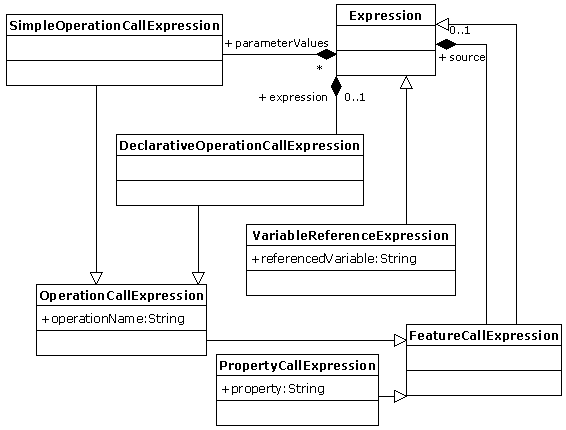
\includegraphics{images/EOLExpressions.png}
	\caption{Overview of the feature navigation EOL expressions}
	\label{fig:EOLExpressions}
\end{figure}

In terms of concrete syntax, `.' is used as a uniform operator to access a property of an object and to invoke an operation on it. The `$\rightarrow$' operator, which is used in OCL to invoke first-order logic operations on sets, has been also preserved for syntax compatibility reasons. In EOL, every operation can be invoked both using the `.' or the '$\rightarrow$' operators, with a slightly different semantics to enable overriding the built-in operations. If the `.' operator is used, precedence is given to the user-defined operations, otherwise precedence is given to the built-in operations. For instance, the Any type defines a println() method that prints the string representation of an object to the standard output stream. In Listing \ref{lst:Expressions}, the user has defined another parameterless println() operation in the context of Any. Therefore the call to println() in Line 1 will be dispatched to the user-defined println() operation defined in line 3. In its body the operation uses the `$\rightarrow$' operator to invoke the built-in println() operation (line 4).

\begin{lstlisting}[float=tbp, caption=Invoking operations using EOL, label=lst:Expressions, language=EOL]
"Something".println();

operation Any println() : Any {
	("Printing : " + self)->println();
}
\end{lstlisting}

\subsection{Arithmetical and Comparison Operators}

EOL provides common operators for performing arithmetical computations and comparisons illustrated in Tables \ref{tab:ArithmeticalOperators} and \ref{tab:ComparisonOperators} respectively.

%Figures \ref{fig:EOLArithmeticalOperators} and \ref{fig:EOLComparisonOperators} respectively.
%
%\begin{figure}
%	\centering
%		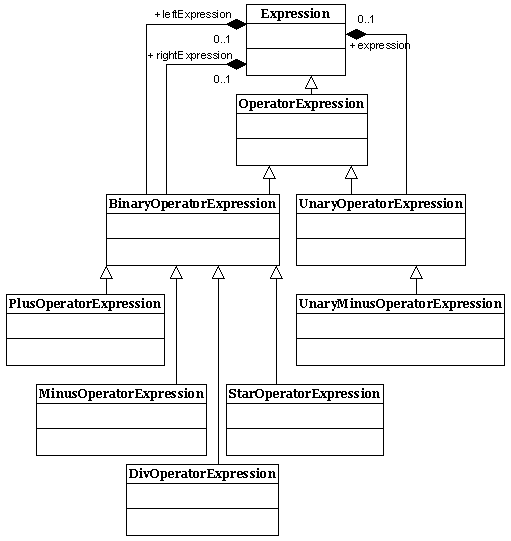
\includegraphics{images/EOLArithmeticalOperators}
%	\caption{Overview of the arithmetical EOL operator expressions}
%	\label{fig:EOLArithmeticalOperators}
%\end{figure}
%
%\begin{figure}
%	\centering
%		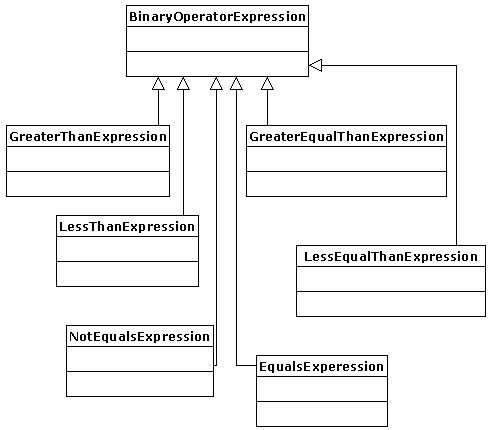
\includegraphics{images/EOLComparisonOperators}
%	\caption{Overview of the comparison EOL operator expressions}
%	\label{fig:EOLComparisonOperators}
%\end{figure}

\begin{longtabu} {|p{3.5cm}|X|}
			
			\caption{Arithmetical operators}
			\label{tab:ArithmeticalOperators}\\
			
			\hline
							
			\textbf{Operator} & \textbf{Description} \\\hline

				$+$ & Adds reals/integers and concatenates strings \\\hline
	
				$-$ & Subtracts reals/integers \\\hline
				
				$-$ (unary) & Returns the negative of a real/integer \\\hline
				
				$*$ & Multiplies reals/integers \\\hline
				
				$/$ & Divides reals/integers \\\hline
				
\end{longtabu}

\clearpage

\begin{longtabu} {|p{3.5cm}|X|}
			
			\caption{Comparison operators}
			\label{tab:ComparisonOperators}\\
			
			\hline
							
			\textbf{Operator} & \textbf{Description} \\\hline

			$=$ & Returns true if the left hand side equals the right hand side. In the case of primitive types (String, Boolean, Integer, Real) the operator compares the values; in the case of objects it returns true if the two expressions evaluate to the same object \\\hline
			
			$<>$ & Is the logical negation of the ($=$) operator \\\hline
				
			$>$ & For reals/integers returns true if the left hand side is greater than the right hand side number \\\hline
			
			$<$ & For reals/integers returns true if the left hand side is less than then right hand side number \\\hline
			
			$>=$ & For reals/integers returns true if the left hand side is greater or equal to the right hand side number \\\hline
			
			$<=$ & For reals/integers returns true if the left hand side is less or equal to then right hand side number \\\hline
		
\end{longtabu}

\subsection{Logical Operators}

EOL provides common operators for performing logical computations illustrated in Table \ref{tab:LogicalOperators}. Logical operations apply only to instances of the Boolean primitive type.

%\begin{figure}
%	\centering
%		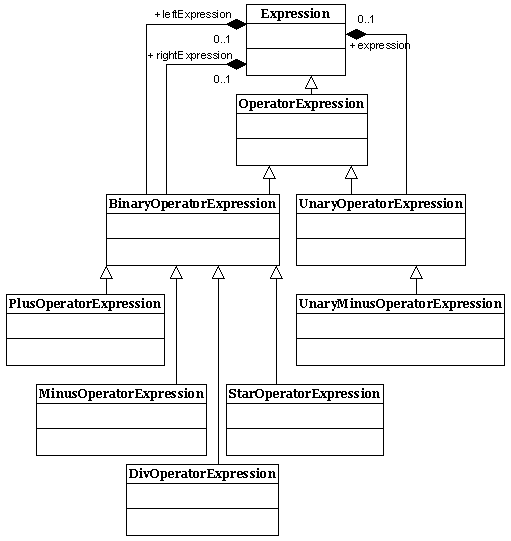
\includegraphics{images/EOLArithmeticalOperators}
%	\caption{Overview of the logical EOL operator expressions}
%	\label{fig:EOLLogicalOperators}
%\end{figure}

\begin{longtabu} {|p{3.5cm}|X|}
			
			\caption{Logical Operators}
			\label{tab:LogicalOperators}\\
			
			\hline
							
			\textbf{Operator} & \textbf{Description} \\\hline

			and & Returns the logical conjunction of the two expressions \\\hline
			
			or & Returns the logical disjunction of the two expressions \\\hline
			
			not & Returns the logical negation of the expression \\\hline
			
			implies & Returns the logical implication of the two expressions. Implication is calculated according to the truth table \ref{tab:ImpliesTruthTable} \\\hline
			
			xor & returns true if only one of the involved expressions evaluates to true  and false otherwise \\\hline
	
\end{longtabu}
	
\begin{longtable} {|l|l|l|} 
	
	\caption{Implies Truth Table}
	\label{tab:ImpliesTruthTable}\\
	
	\hline
		\textbf{Left} & \textbf{Right} & \textbf{Result} \\\hline
		true & true & true \\\hline
		true & false & false \\\hline
		false & true & true \\\hline
		false & false & true \\\hline			

\end{longtable}

\subsection{Enumerations}

EOL provides the \# operator for accessing enumeration literals. For example, the VisibilityEnum\#vk\_public expression returns the value of the literal \emph{vk\_public} of the \emph{VisibilityEnum} enumeration. For EMF metamodels, \emph{VisibilityEnum\#vk\_public.instance} can also be used.

\section{Statements}

\subsection{Variable Declaration Statement}

A variable declaration statement declares the name and (optionally) the type and initial value of a variable in an EOL program. If no type is explicitly declared, the variable is assumed to be of type Any. For variables of primitive type, declaration automatically creates an instance of the type with the default values presented in Table \ref{tab:DefaultValuesOfPrimitiveTypes}. For non-primitive types the user has to explicitly assign the value of the variable either by using the \emph{new} keyword or by providing an initial value expression. If neither is done the value of the variable is undefined. Variables in EOL are strongly-typed. Therefore a variable can only be assigned values that conform to its type (or a sub-type of it).

\begin{table}
  \centering
  \caption{Default values of primitive types}
  \label{tab:DefaultValuesOfPrimitiveTypes}
  \begin{tabular}{|l|l|}
    \hline
    \textbf{Type} & \textbf{Default value} \\\hline
    Integer       & 0                      \\\hline
    Boolean       & false                  \\\hline
    String        & ""                     \\\hline
    Real          & 0.0                    \\\hline
  \end{tabular}
\end{table}

\paragraph{Scope} The scope of variables in EOL is generally limited to the block of statements where they are defined, including any nested blocks. Nevertheless, as discussed in the sequel, there are cases in task-specific languages that build atop EOL where the scope of variables is expanded to other non-nested blocks as well. EOL also allows variable shadowing; that is to define a variable with the same name in a nested block that overrides a variable defined in an outer block. 

In Listing \ref{lst:Variables}, an example of declaring and using variables is provided. Line 1 defines a variable named \emph{i} of type \emph{Integer} and assigns it an initial value of \emph{5}. Line 2 defines a variable named \emph{c} of type \emph{Class} (from model Uml) and creates a new instance of the type in the model (by using the \emph{new} keyword). The commented out assignment statement of line 3 would raise a runtime error since it would attempt to assign a \emph{String} value to an \emph{Integer} variable. The condition of line 4 returns true since the \emph{c} variable has been initialized before. Line 5 defines a new variable also named \emph{i} that is of type \emph{String} and which overrides the \emph{Integer} variable declared in line 1. Therefore the assignment statement of line 6 is legitimate as it assigns a string value to a variable of type String. Finally, as the program has exited the scope of the \emph{if} statement, the assignment statement of line 7 is also legitimate as it refers to the \emph{i} variable defined in line 1.

\begin{lstlisting}[float=tbp, caption=Example illustrating declaration and use of variables, label=lst:Variables, language=EOL]
var i : Integer = 5;
var c : new Uml!Class;
//i = "somevalue";
if (c.isDefined()) {
	var i : String;
	i = "somevalue";
}
i = 3;
\end{lstlisting}

\subsection{Assignment Statement}

The assignment statement is used to update the values of variables and  properties of native objects and model elements.

\paragraph{Variable Assignment}

When the left hand side of an assignment statement is a variable, the value of the variable is updated to the object to which the right hand side evaluates to. If the type of the right hand side is not compatible (kind-of relationship) with the type of the variable, the assignment is illegal and a runtime error is raised. Assignment to objects of primitive types is performed by value while assignment to instances of non-primitive values is performed by reference. For example, in Listing \ref{lst:VariableAssignmentByReference}, in line 1 the value
of the a variable is set to a new Class in the Uml model. In line 2, a new untyped variable b is declared and its value is assigned to a. In line 3 the name of the class is updated to Customer and thus, line 4 prints Customer to the standard output stream. On the other hand, in Listing \ref{lst:VariableAssignmentByValue}, in line 1 the a String variable is declared. In line 2 an untyped variable b is declared. In line 3, the value of a is changed to Customer (which is an instance of the primitive \emph{String} type). This has no effect on b and thus line 4 prints an empty string to the standard output stream.

\begin{lstlisting}[float=tbp, caption=Assigning the value of a variable by reference, label=lst:VariableAssignmentByReference, language=EOL]
var a : new Uml!Class;
var b = a;
a.name = "Customer";
b.name.println();
\end{lstlisting}

\begin{lstlisting}[float=tbp, caption=Assigning the value of a variable by value, label=lst:VariableAssignmentByValue, language=EOL]
var a : String;
var b = a;
a = "Customer";
b.println();
\end{lstlisting}

\paragraph{Native Object Property Assignment}

When the left hand side of the assignment is a property of a native object, deciding on the legality and providing the semantics of the assignment is delegated to the execution engine. For example, in a Java-based execution engine, given that x is a native object, the statement \emph{x.y = a} may be interpreted as \emph{x.setY(a)} or if x is an instance of a map \emph{x.put(''y'',a)}. By contrast, in a C\# implementation, it can be interpreted as \emph{x.y = a} since
the language natively supports properties in classes.

\paragraph{Model Element Property Assignment}

When the left hand side of the assignment is a property of a model element, the model that owns the particular model element (accessible using the \emph{ModelRepository.getOwningModel() }operation) is responsible for implementing the semantics of the assignment using its associated \emph{propertyGetter} as discussed in Section \ref{sec:Design.EMC.CRUD}. For example, if x is a model element, the statement \emph{x.y = a} may be interpreted using the Java code of Listing \ref{lst:EmfModelElementPropertyAssignment} if x belongs to an EMF-based model or using the Java code of Listing \ref{lst:MdrModelElementPropertyAssignment} if it belongs to an MDR-based model.

\begin{lstlisting}[float=tbp, caption=Java code that assigns the value of a property of a model element that belongs to an EMF-based model, label=lst:EmfModelElementPropertyAssignment, language=Java]
EStructuralFeature feature = x.eClass().getEStructuralFeature("y");
x.eSet(feature, a);
\end{lstlisting}

\begin{lstlisting}[float=tbp, caption=Java code that assigns the value of a property of a model element that belongs to an MDR-based model, label=lst:MdrModelElementPropertyAssignment, language=Java]
StructuralFeature feature = findStructuralFeature(x.refClass(), "y");
x.refSetValue(feature, a);
\end{lstlisting}

\subsection{Special Assignment Statement}
\label{sec:Design.EOL.SpecialAssignmentStatement}
In task-specific languages, an assignment operator with task-specific semantics is often required. Therefore, EOL provides an additional assignment operator. In standalone EOL, the operator has the same semantics with the primary assignment operator discussed above, however task-specific languages can redefine its semantics to implement custom
assignment behaviour. For example, consider the simple model-to-model transformation of Listing \ref{lst:SpecialAssignmentStatement} where a simple object oriented model is transformed to a simple database model using an ETL (see Section \ref{sec:ETL}) transformation. The Class2Table rule transforms a Class of the OO model into
a Table in the DB model and sets the name of the table to be the same as the name of the class. Rule Atribute2Column transforms an Attribute from the OO model into a column in the DB model. Except for setting its name (line 12), it also needs to define that the column belongs to the table which corresponds to the class that defines the source attribute. The commented-out assignment statement of line 13 cannot
be used for this purpose since it would illegaly attempt to assign the owningTable feature of the column to a model element of an inappropriate type (OO!Class). However, the special assignment operator in the task-specific language implements the semantics discussed in Section \ref{sec:Design.ETL.SpecialAssignmentOperator}, and thus in line 14 it assigns to the owningTable feature not the class that owns the attribute but its corresponding table (calculated using the Class2Table rule) in the DB model. 

\begin{lstlisting}[float=tbp, caption=A simple model-to-model transformation
demonstrating the special assignment statement, label=lst:SpecialAssignmentStatement, language=ETL]
rule Class2Table
  transform c : OO!Class
  to t : DB!Table {
  
  t.name = c.name;
}

rule Attribute2Column
  transform a : OO!Attribute
  to c : DB!Column {
  
  c.name = a.name;
  //c.owningTable = c.owningClass;
  c.owningTable ::= c.owningClass;
}

\end{lstlisting}

\subsection{If Statement}

As in most programming languages, an if statement consists of a condition, a block of statements that is executed if the condition is satisfied and (optionally) a block of statements that is executed otherwise. As an example, in Listing \ref{lst:IfStatement}, if variable a holds a value that is greater than 0 the statement of line 3 is executed, otherwise the statement of line 5 is executed.

\begin{lstlisting}[float=h, caption=Example illustrating an if statement, label=lst:IfStatement, language=EOL]
if (a > 0) {
	"A is greater than 0".println();
}
else { "A is less equal than 0".println(); }
\end{lstlisting}

\subsection{Switch Statement}

A switch statement consists of an expression and a set of cases, and can be used to implement multi-brancing. Unlike Java/C, switch in EOL doesn't by default fall through to the next case after a successful one. Therefore, it is not necessary to add a \emph{break} statement after each case. To enable falling through to the next case you can use the \emph{continue} statement. Also, unlike Java/C, the switch expression can return anything (not only integers). As an example, when executed, the code in Listing \ref{lst:SwitchStatement1} prints 2 while the code in Listing \ref{lst:SwitchStatement2} prints 2,3,default.

\begin{lstlisting}[float=h, caption=Example illustrating a switch statement, label=lst:SwitchStatement1, language=EOL]
var i = "2";

switch (i) {
	case "1" : "1".println(); 
	case "2" : "2".println();
	case "3" : "3".println();
	default : "default".println(); 
}
\end{lstlisting}

\begin{lstlisting}[float=h, caption=Example illustrating falling through cases in a switch statement, label=lst:SwitchStatement2, language=EOL]
var i = "2";

switch (i) {
	case "1" : "1".println(); 
	case "2" : "2".println(); continue;
	case "3" : "3".println();
	default : "default".println(); 
}
\end{lstlisting}

\subsection{While Statement}
\label{sec:while-statement}

A while statement consists of a condition and a block of statements which are executed as long as the condition is satisfied. For example, in Listing \ref{lst:WhileStatement} the body of the while statement is executed 5 times printing the numbers 0 to 4 to the output console. Inside the body of a \emph{while} statement, the built-in read-only \emph{loopCount} integer variable holds the number of times the innermost loop has been executed so far (including the current iteration). Right after entering the loop for the first time and before running the first statement in its body, \emph{loopCount} is set to 1, and it is incremented after each following iteration.

\begin{lstlisting}[float=h, caption=Example of a while statement, label=lst:WhileStatement, numbers=left, language=EOL]
var i : Integer = 0;
while (i < 5) {
  // both lines print the same thing
  i.println();
  (loopCount - 1).println();
  // increment the counter
  i = i+1;
}
\end{lstlisting}

\subsection{For Statement}

In EOL, for statements are used to iterate the contents of collections. A for statement defines a typed iterator and an iterated collection as well as a block of statements that is executed for every item in the collection that has a kind-of relationship with the type defined by the iterator. As with the majority of programming languages, modifying a collection while iterating it raises a runtime error. To avoid this situation, users can use the clone() built-in operation of the Collection type discussed in \ref{sec:Design.EOL.Collections}. 

\begin{lstlisting}[float=h, caption=Example of a for statement, label=lst:ForStatement, language=EOL]
var col : Sequence = Sequence{"a", 1, 2, 2.5, "b"};
for (r : Real in col) {
	r.print();
	if (hasMore){",".print();}
}
\end{lstlisting}

Inside the body of a \emph{for} statement two built-in read-only variables are visible: the \emph{loopCount} integer variable (explained in Section~\ref{sec:while-statement}) and the \emph{hasMore} boolean variable. \emph{hasMore} is used to determine if there are more items if the collection for which the loop will be executed. For example, in Listing \ref{lst:ForStatement} the col heterogeneous Sequence is defined that contains two strings (a and b), two integers (1,2) and one real (2.5). The for loop of line 2 only iterates through the items of the collection that are of kind Real and therefore prints 1,2,2.5 to the standard output stream.

\begin{lstlisting}[float=h, caption=Example of a for statement, label=lst:TransactionStatement, language=EOL]
var system : System.allInstances.first();

for (i in Sequence {1..100}) {

	transaction {
		
		var failedProcessors : Set; 
		
		while (failedProcessors.size() < 10) {
			failedProcessors.add(system.processors.random());
		}
		
		for (processor in failedProcessors) {
			processor.failed = true;
			processor.moveTasksElsewhere();
		}
		
		system.evaluateAvailability();
		
		abort; /*@\label{line:Abort}@*/
	}
	
}
\end{lstlisting}

\begin{lstlisting}[float=h, caption=Calculating and printing the depth of each Tree, label=lst:NoExtendedProperties, language=EOL]
var depths = new Map; /*@\label{line:DeclareMap}@*/

for (n in Tree.allInstances.select(t|not t.parent.isDefined())) {
	n.setDepth(0);
}

for (n in Tree.allInstances) {
	(n.name + " " + depths.get(n)).println();
}

operation Tree setDepth(depth : Integer) {
	depths.put(self,depth); /*@\label{line:PutDepthInMap}@*/
	for (c in self.children) {
		c.setDepth(depth + 1);
	}
}
\end{lstlisting}

\subsection{Break, BreakAll and Continue Statements}

To exit from for and while loops on demand, EOL provides the break and breakAll statements. The break statement exits the innermost loop while the breakAll statement exits all outer loops as well. On the other hand, to skip a particular loop and proceed with the next one, EOL provides the continue statement. For example, the excerpt of Listing \ref{lst:BreakStatement}, prints \textit{2,1 3,1} to the standard output stream.

\begin{lstlisting}[float=h, caption=Example of the break\, breakAll and continue statements, label=lst:BreakStatement, language=EOL]
for (i in Sequence{1..3}) {
	if (i = 1) {continue;}
	for (j in Sequence{1..4}) {
		if (j = 2) {break;}
		if (j = 3) {breakAll;}
		(i + "," + j).println();
	}
}
\end{lstlisting}

\subsection{Throw Statement}
\label{sec:eol-throw}

EOL provides the throw statement for throwing a value as an \class{EolUserException} Java exception. This is especially useful when invoking EOL scripts from Java code: by catching and processing the exception, the Java code may be able to automatically handle the problem without requiring user input. Any value can be thrown, as shown in Listing~\ref{lst:ThrowStatement}, where we throw a number and a string.

\begin{lstlisting}[float=h, caption=Example of the throw statement, label=lst:ThrowStatement, language=EOL]
throw 42;
throw "Error!";
\end{lstlisting}

\subsection{Transaction Statement}

As discussed in Section \ref{sec:EMC.ModelTransactionSupport}, the underlying EMC layer provides support for transactions in models. To utilize this feature EOL provides the transaction statement. A transaction statement (optionally) defines the models that participate in the transaction. If no models are defined, it is assumed that all the models that are accessible from the enclosing program participate. When the statement is executed, a transaction is started on each participating model. If no errors are raised during the execution of the contained statements, any changes made to model elements are committed. On the other hand, if an error is raised the transaction is rolled back and any changes made to the models in the context of the transaction are undone. The user can also use the abort statement to explicitly exit a transaction and roll-back any changes done in its context. In Listing \ref{lst:TransactionStatement}, an example of using this feature in a simulation problem is illustrated.

In this problem, a system consists of a number of processors. A processor manages some tasks and can fail at any time. The EOL program in Listing \ref{lst:TransactionStatement} performs 100 simulation steps, in every one of which 10 random processors from the model (lines 7-11) are marked as failed by setting their \emph{failed} property to true (line 14). Then, the tasks that the failed processors manage are moved to other processors (line 15). Finally the availability of the system in this state is evaluated.

After a simulation step, the state of the model has been drastically changed since processors have failed and tasks have been relocated. To be able to restore the model to its original state after every simulation step, each step is executed in the context of a transaction which is explicitly aborted (line \ref{line:Abort}) after evaluating the availability of the system. Therefore after each simulation step the model is restored to its original state for the next step to be executed.



\section{Extended Properties}
\label{sec:ExtendedProperties}

Quite often, during a model management operation it is necessary to associate model elements with information that is not supported by the metamodel they conform to. For instance, the EOL program in listing \ref{lst:NoExtendedProperties} calculates the depth of each Tree element in a model that conforms to the Tree metamodel displayed in Figure \ref{fig:Tree1}.

\begin{figure}[t!]
	\centering
		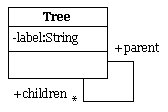
\includegraphics{images/metamodels/Tree.png}
	\caption{The Tree Metamodel}
	\label{fig:Tree1}
\end{figure}

As the Tree metamodel doesn't support a \emph{depth} property in the Tree metaclass, each Tree has to be associated with its calculated depth (line \ref{line:PutDepthInMap}) using the \emph{depths} map defined in line \ref{line:DeclareMap}. Another approach would be to extend the Tree metamodel to support the desired \emph{depth} property; however, applying this technique every time an additional property is needed for some model management operation would quickly pollute the metamodel with properties of secondary importance.

To simplify the code required in such cases, EOL provides the concept of \emph{extended properties}. In terms of concrete syntax, an extended property is a normal property, the name of which starts with the tilde character (\verb|~|). With regards to its execution semantics, the first time the value of an extended property of an object is assigned, the property is created and associated with the object. Then, the property can be accessed as a normal property. If an extended property is accessed before it is assigned, it returns \emph{null}. Listing \ref{lst:ExtendedProperties} demonstrates using a $~$\emph{depth} extended property to eliminate the need for using the \emph{depths} map in Listing \ref{lst:NoExtendedProperties}.

\begin{lstlisting}[float=tbp, caption=A simplified version of Listing \ref{lst:NoExtendedProperties} using extended properties, label=lst:ExtendedProperties, language=EOL]
for (n in Tree.allInstances.select(t|not t.parent.isDefined())) {
	n.setDepth(0);
}

for (n in Tree.allInstances) {
	(n.name + " " + n.~depth).println();
}

operation Tree setDepth(depth : Integer) {
	self.~depth = depth;
	for (c in self.children) {
		c.setDepth(depth + 1);
	}
}
\end{lstlisting}

%\section{Annotations}
%\label{sec:Design.EOL.Annotations}

\section{Context-Independent User Input}
\label{sec:Design.EOL.UserInput}

A common assumption in model management languages is that model management tasks are only executed in a batch-manner without human intervention. However, as demonstrated in the sequel, it is often useful for the user to provide feedback that can precisely drive the execution of a model management operation.

Model management operations can be executed in a number of runtime environments in each of which a different user-input method is more appropriate. For instance when executed in the context of an IDE (such as Eclipse) visual dialogs are preferable, while when executed in the context of a server or from within an ANT workflow, a command-line user input interface is deemed more suitable. To abstract away from the different runtime environments and enable the user to specify user interaction statements uniformly and regardless of the runtime context, EOL provides the \emph{IUserInput} interface that can be realized in different ways according to the execution environment and attached to the runtime context via the \emph{IEolContext.setUserInput(IUserInput userInput)} method. The \emph{IUserInput} specifies the methods presented in Table \ref{tab:IUserInputOperations}.

\begin{longtabu} {|p{6.5cm}|X|}
			
			\caption{Operations of IUserInput}
			\label{tab:IUserInputOperations}\\
			
			\hline
							
			\textbf{Signature} & \textbf{Description} \\\hline

			inform(message : String) & Displays the specified message to the user\\\hline
			
			confirm(message : String, [default : Boolean]) : Boolean & Prompts the user to confirm if the condition described by the message holds \\\hline
			
			prompt(message : String, [default : String]) : String & Prompts the user for a string in response to the message \\\hline
			
			promptInteger(message : String, [default : Integer]) : Integer & Prompts the user for an Integer \\\hline
			
			promptReal(message : String, [default : Real]) : Real & Prompts the user for a Real \\\hline
			
	 		choose(message : String, options : Sequence, [default : Any]) : Any & Prompts the user to select one of the options \\\hline
			
			chooseMany(message : String, options : Sequence, [default : Sequence]) : Sequence & Prompts the user to select one or more of the options \\\hline
			
\end{longtabu}

As displayed above, all the methods of the \emph{IUserInput} interface accept a \emph{default} parameter. The purpose of this parameter is dual. First, it enables the designer of the model management program to prompt the user with the most likely value as a default choice and secondly it enables a concrete implementation of the interface (\emph{UnattendedExecutionUserInput}) which returns the default values without prompting the user at all and thus, can be used for unattended execution of interactive Epsilon programs. Figures \ref{fig:EclipseUserInput} and \ref{fig:ConsoleUserInput} demonstrate the interfaces through which input is required by the user when the exemplar \emph{System.user.promptInteger('Please enter a number', 1);} statement is executed using  an Eclipse-based and a command-line-based \emph{IUserInput} implementation respectively.

\begin{figure}[b!]
	\centering
		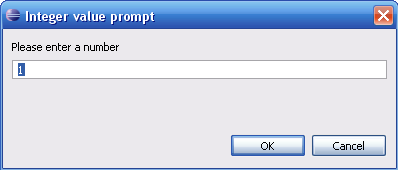
\includegraphics{images/EclipseUserInput.png}
	\caption{Example of an Eclipse-based IUserInput implementation}
	\label{fig:EclipseUserInput}
\end{figure}

\begin{figure}
	\centering
		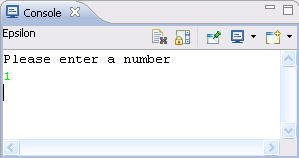
\includegraphics{images/ConsoleUserInput.png}
	\caption{Example of a command-line-based IUserInput implementation}
	\label{fig:ConsoleUserInput}
\end{figure}

User-input facilities have been found to be particularly useful in all model management tasks. Such facilities are essential for performing operations on live models such as model validation and model refactoring but can also be useful in model comparison where marginal matching decisions can be delegated to the user and model transformation where the user can interactively specify the elements that will be transformed into corresponding elements in the target model. Examples of interactive model management operations that make use of the input facilities provided by EOL are demonstrated in Sections \ref{sec:InteractiveModelTransformation} and \ref{sec:InteractiveModelComparison}
